\chapter{Reproducción sexual de los mamíferos}\label{ch:b2:mammal-reproduction}

Un óvulo humano mide una décima de milímetro, la célula más grande del
cuerpo; un espermatozoide es un núcleo con una hélice, uno de los
trescientos millones liberados de una vez, de los cuales unas pocas
decenas llegarán al óvulo y uno entrará en él. En una semana el óvulo
fecundado se ha convertido en una esfera hueca que se hunde en la pared
del útero y construye, con sus propias células externas, un órgano ---
la \omterm{def:b2:mammal-reproduction:placenta}{placenta} --- a través del cual su madre lo alimentará durante nueve
meses. Después nace y se alimenta de leche. Todos los mamíferos lo
hacen; ningún otro animal lo hace todo. Este capítulo sigue a los gametos
hasta la fecundación, al embrión hasta la \omterm{def:b2:mammal-reproduction:implantation}{implantación} y al organismo a
lo largo de la gestación, el parto y la lactancia, y termina con la
manera en que se forman los dos sexos.

\section{Gónadas y gametos}

\begin{definition}[El testículo y la espermatogénesis]\label{def:b2:mammal-reproduction:testis}
\index{espermatogénesis}\index{túbulo seminífero}\index{célula de Sertoli}\index{célula de Leydig}
El \emph{testículo} es una masa de \emph{túbulos seminíferos}, de varios
cientos de metros en total, cuyas paredes producen espermatozoides; entre
los túbulos se sitúan las \emph{células de Leydig}, que producen
testosterona. En la pared del túbulo, las \emph{espermatogonias} del
borde externo se dividen por mitosis, mantienen una población de células
madre y envían células hacia dentro; estas crecen y dan
\emph{espermatocitos} primarios, que realizan la \omterm{def:b2:meiosis-heredity:meiosis}{meiosis} I (y dan dos
espermatocitos secundarios) y la \omterm{def:b2:meiosis-heredity:meiosis}{meiosis} II (y dan cuatro
\emph{espermátidas} \omterm{def:b2:meiosis-heredity:meiosis}{haploides}); las espermátidas pierden la mayor parte
de su citoplasma, condensan su núcleo, forman un flagelo y cubren el
núcleo con el \emph{acrosoma}, una vesícula de enzimas, para convertirse
en \emph{espermatozoides}, que se liberan a la luz del túbulo. Grandes
\emph{células de Sertoli} atraviesan la pared, nutren a las células
germinales y forman, mediante uniones estrechas entre ellas, una
\emph{barrera hematotesticular} que aleja el sistema inmunitario de unas
células que solo aparecen en la pubertad. Toda la secuencia dura unos
\num{64} días en el hombre y produce unos $10^{8}$ espermatozoides al día
desde la pubertad hasta la vejez. Los espermatozoides salen del testículo
inmóviles y maduran en el \emph{epidídimo} durante dos semanas.
\end{definition}

\begin{omfigure}
\begin{tikzpicture}[every node/.style={font=\scriptsize}]
  % tubule cross-section: concentric layers
  \draw[thick, fill=omExo!15] (0,0) circle (2.5);
  \draw[thick, fill=omExo!8] (0,0) circle (2.2);
  \draw[thick, fill=omDef!10] (0,0) circle (1.6);
  \draw[thick, fill=omProp!12] (0,0) circle (1.0);
  \draw[thick, fill=white] (0,0) circle (0.45);
  % cells
  \foreach \a in {0,30,...,330} \draw[thick, fill=omDef!40] (\a:2.0) circle (0.13);
  \foreach \a in {15,45,...,345} \draw[thick, fill=omDef!70] (\a:1.32) circle (0.16);
  \foreach \a in {0,20,...,340} \draw[thick, fill=omProp!60] (\a:0.75) circle (0.08);
  \foreach \a in {10,40,...,340} \draw[thick, omProp!80!black] (\a:0.45) -- (\a:0.15);
  % Sertoli cell: tall wedge
  \draw[thick, omExo!70!black, fill=omExo!40, opacity=0.6] (100:2.2) .. controls (90:1.6) and (95:0.9) .. (92:0.5) .. controls (80:0.9) and (75:1.6) .. (72:2.2) -- cycle;
  % Leydig cells outside
  \foreach \p in {(2.9,0.8),(3.1,0.3),(2.8,-0.3)} \draw[thick, fill=omThm!40] \p circle (0.14);
  % labels
  \draw (2.0,0) -- (3.6,-0.5) node[right, align=left] {espermatogonias ($2n$)\\en el borde externo};
  \draw (1.32,-0.7) -- (3.6,-1.5) node[right, align=left] {espermatocitos primarios\\(meiosis I)};
  \draw (0.75,-0.4) -- (3.6,-2.4) node[right, align=left] {espermátidas ($n$)};
  \draw (0.3,-0.2) -- (3.6,-3.1) node[right, align=left] {espermatozoides en la luz};
  \draw (2.95,0.55) -- (3.6,0.6) node[right, align=left] {células de Leydig:\\testosterona};
  \draw (88:1.4) -- (3.6,1.8) node[right, align=left] {célula de Sertoli que atraviesa la pared};
  \node[anchor=east, align=right] at (-2.7,0) {exterior\\(lámina basal)};
\end{tikzpicture}

{\small Un \omterm{def:b2:mammal-reproduction:testis}{túbulo seminífero} en sección transversal. Las células
germinales maduran desde la pared externa (espermatogonias) hacia dentro
(espermatocitos, espermátidas, espermatozoides en la luz), sostenidas por
las \omterm{def:b2:mammal-reproduction:testis}{células de Sertoli}; las \omterm{def:b2:mammal-reproduction:testis}{células de Leydig}, entre los túbulos,
producen testosterona.}
\end{omfigure}

\begin{omfigure}
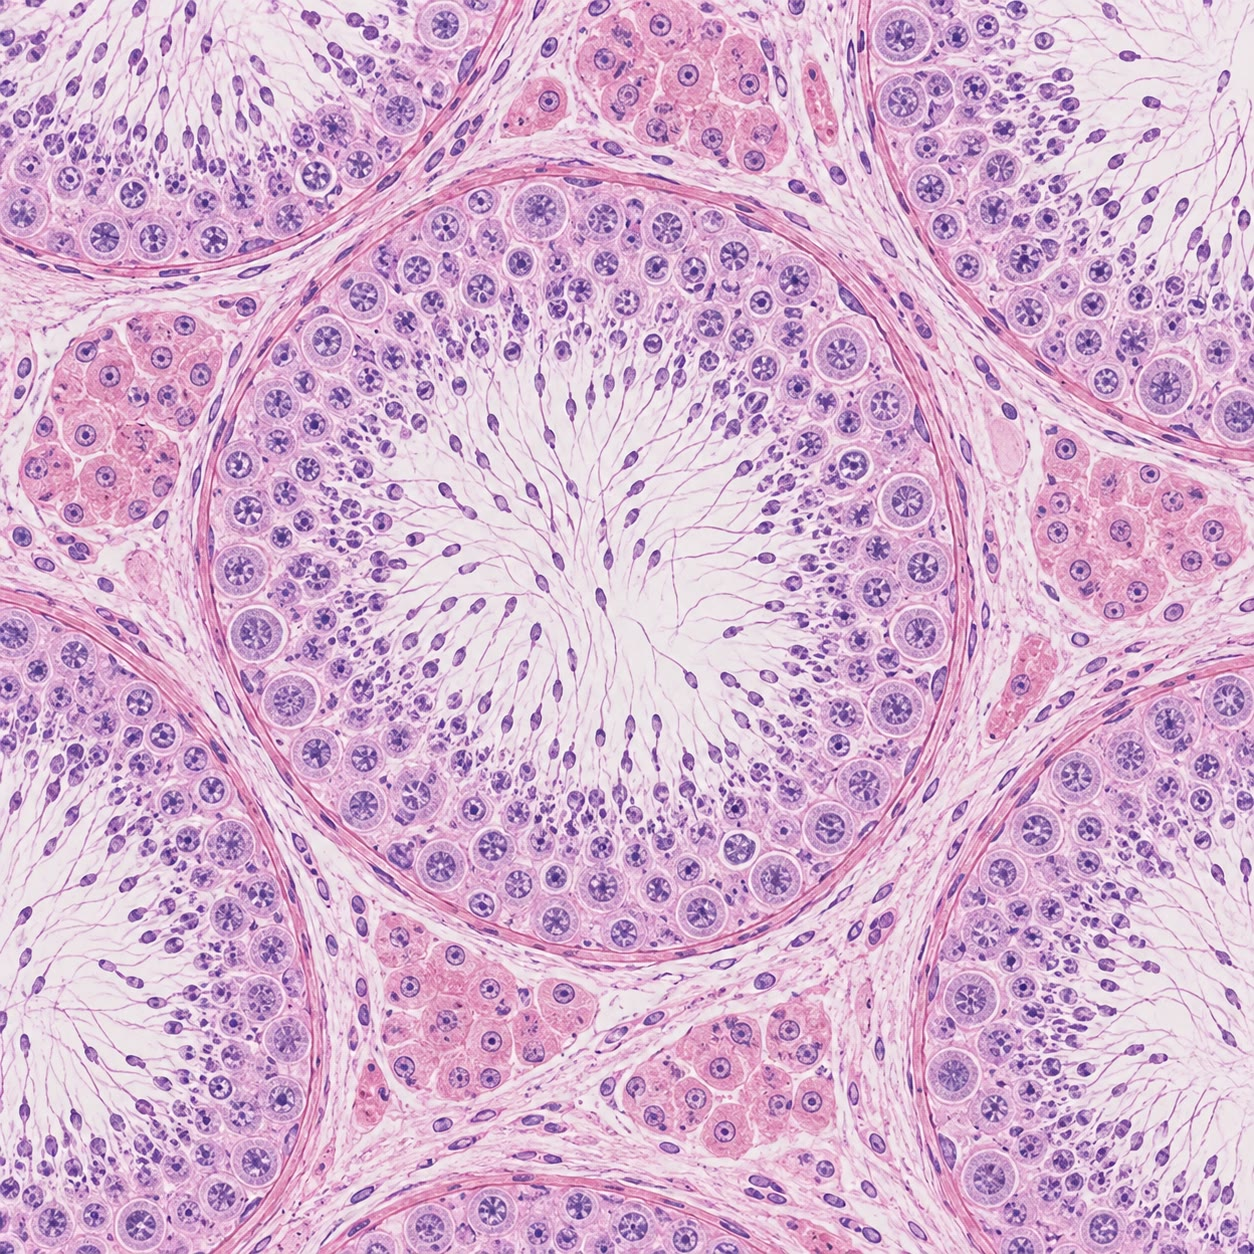
\includegraphics[width=0.42\linewidth]{images/book4/ai/b4-08-testis-histology.jpg}\hspace{0.04\linewidth}
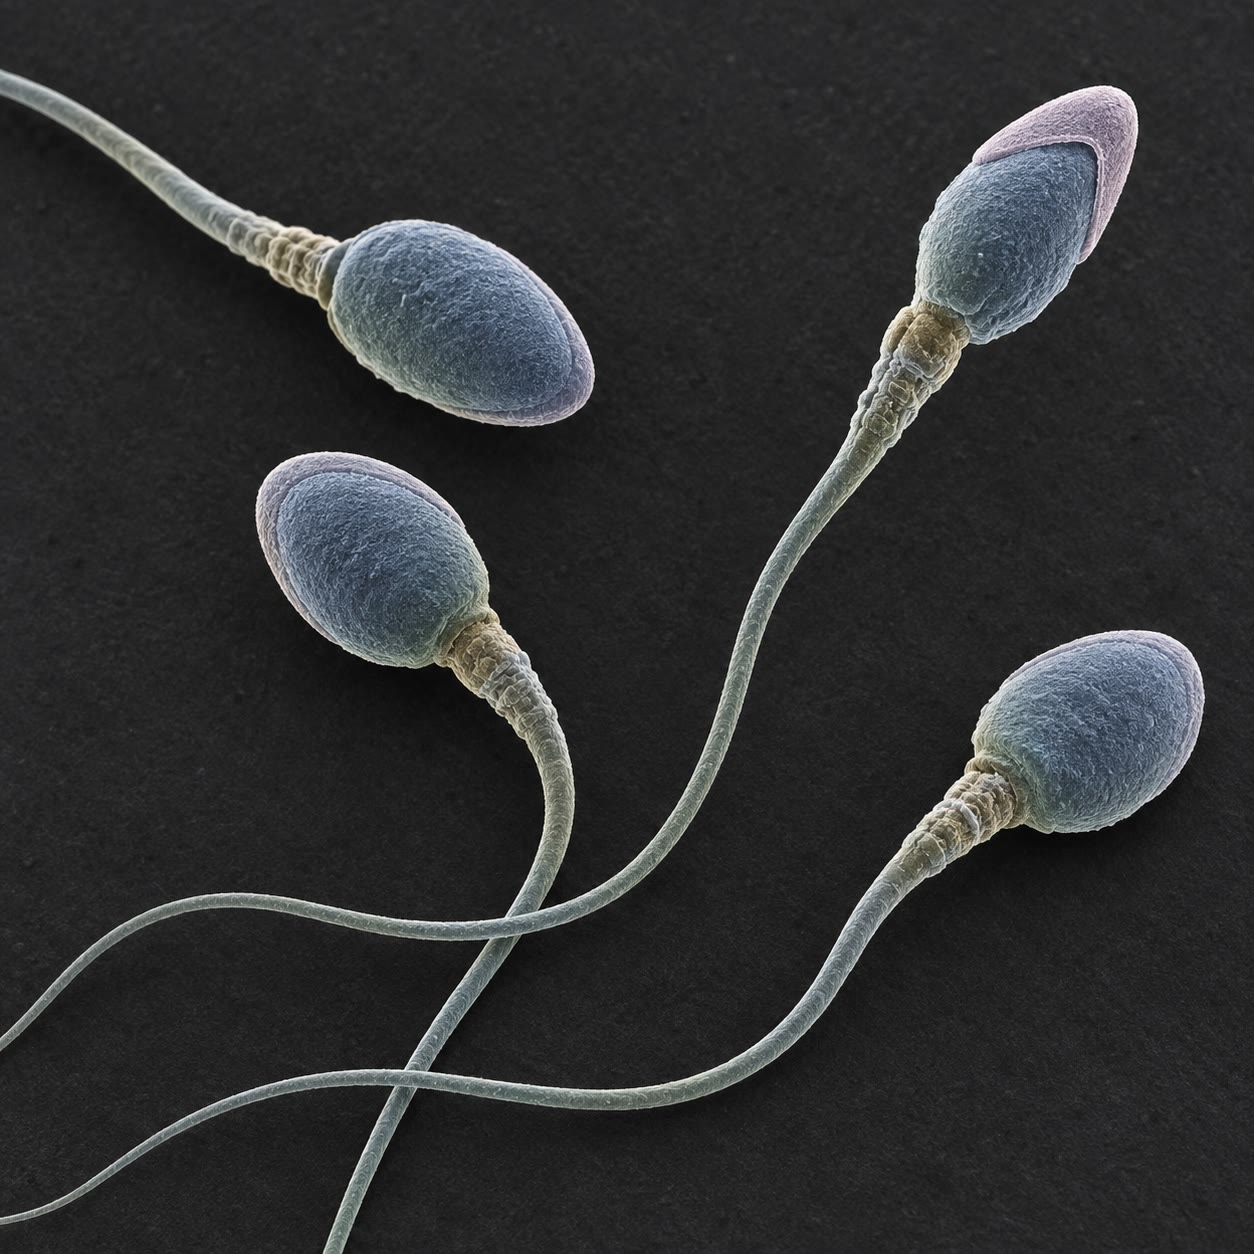
\includegraphics[width=0.42\linewidth]{images/book4/ai/b4-08-sperm-sem.jpg}

{\small Izquierda: \omterm{def:b2:mammal-reproduction:testis}{túbulos seminíferos} en sección, con las células
germinales dispuestas en capas desde la pared hasta la luz. Derecha:
espermatozoides al microscopio electrónico de barrido, con el capuchón
acrosómico visible en las cabezas.}
\end{omfigure}

\begin{definition}[El ovario y la ovogénesis]\label{def:b2:mammal-reproduction:ovary}
\index{ovogénesis}\index{folículo}\index{ovulación}\index{cuerpo lúteo}
La ovogénesis es, en casi todos los aspectos, la imagen especular de la
\omterm{def:b2:mammal-reproduction:testis}{espermatogénesis}. Las \emph{ovogonias} solo se multiplican en el feto: al
nacer, una niña lleva una reserva de alrededor de un millón de
\emph{ovocitos} primarios, cada uno detenido en la \omterm{prop:b2:meiosis-heredity:stages}{profase I} de la
\omterm{def:b2:meiosis-heredity:meiosis}{meiosis} y envuelto en una sola capa de células --- un \emph{folículo
primordial} ---, y nunca se forman otros nuevos. Desde la pubertad, cada
mes crece una cohorte de folículos: el ovocito aumenta de tamaño, las
células de la \emph{granulosa} que lo rodean se multiplican en capas, se
forma una \emph{teca} externa, se abre una cavidad llena de líquido (el
\emph{folículo de De Graaf}, de dos centímetros de diámetro), y
normalmente uno solo llega a la \emph{ovulación}: el ovocito, que solo
ahora completa la \omterm{def:b2:meiosis-heredity:meiosis}{meiosis} I y vuelve a detenerse en la metafase II, es
expulsado con su halo de células de la granulosa hacia el oviducto. El
folículo vacío se convierte en el \emph{cuerpo lúteo}, una glándula
temporal de progesterona. La \omterm{def:b2:meiosis-heredity:meiosis}{meiosis} produce un óvulo y tres diminutos
cuerpos polares --- todo el citoplasma va a una sola célula ---, y la
\omterm{def:b2:meiosis-heredity:meiosis}{meiosis} II solo se completa si entra un espermatozoide. Del millón de
ovocitos, unos \num{400} se ovulan a lo largo de la vida; el resto
degenera (\emph{atresia}), y cuando la reserva se agota, hacia los
cincuenta años, los ciclos cesan: la menopausia.
\end{definition}

\begin{omfigure}
\begin{tikzpicture}[every node/.style={font=\scriptsize}, >=stealth]
  % timeline of oogenesis vs spermatogenesis
  \draw[thick, ->] (0,3.0) -- (12.6,3.0); \node[anchor=west] at (12.6,3.0) {edad};
  \foreach \x/\l in {0/{feto}, 2.2/{nacimiento}, 4.6/{pubertad}, 10.2/{$\sim$50 años}}
    \draw (\x,3.1) -- (\x,2.9) node[above=0.15cm] {\l};
  % oogenesis line
  \node[anchor=east, omThm] at (-0.2,1.5) {ovogénesis};
  \draw[very thick, omThm] (0,1.5) -- (1.6,1.5); \node[above, omThm, align=center] at (0.8,1.55) {las ovogonias\\se multiplican};
  \draw[very thick, omThm, dashed] (1.6,1.5) -- (4.6,1.5); \node[below, omThm] at (3.1,1.45) {detención en profase I};
  \draw[very thick, omThm] (4.6,1.5) -- (10.2,1.5); \node[above, omThm, align=center] at (7.4,1.55) {una ovulación al mes;\\meiosis I completada en la ovulación, II en la fecundación};
  \fill[omThm] (10.2,1.5) circle (0.07); \node[below, omThm] at (10.2,1.45) {reserva agotada};
  % spermatogenesis line
  \node[anchor=east, omDef] at (-0.2,0.3) {espermatogénesis};
  \draw[very thick, omDef, dashed] (0,0.3) -- (4.6,0.3); \node[above, omDef] at (2.3,0.35) {espermatogonias en reposo};
  \draw[very thick, omDef, ->] (4.6,0.3) -- (12.6,0.3); \node[above, omDef] at (8.6,0.35) {continua, desde células madre: $10^{8}$ al día, 64 días cada uno};
\end{tikzpicture}

{\small Las dos gametogénesis en el tiempo. Los ovocitos se forman todos
antes del nacimiento y se liberan de uno en uno a partir de una reserva
finita; los espermatozoides se producen continuamente a partir de
células madre durante toda la vida adulta.}
\end{omfigure}

\begin{omfigure}
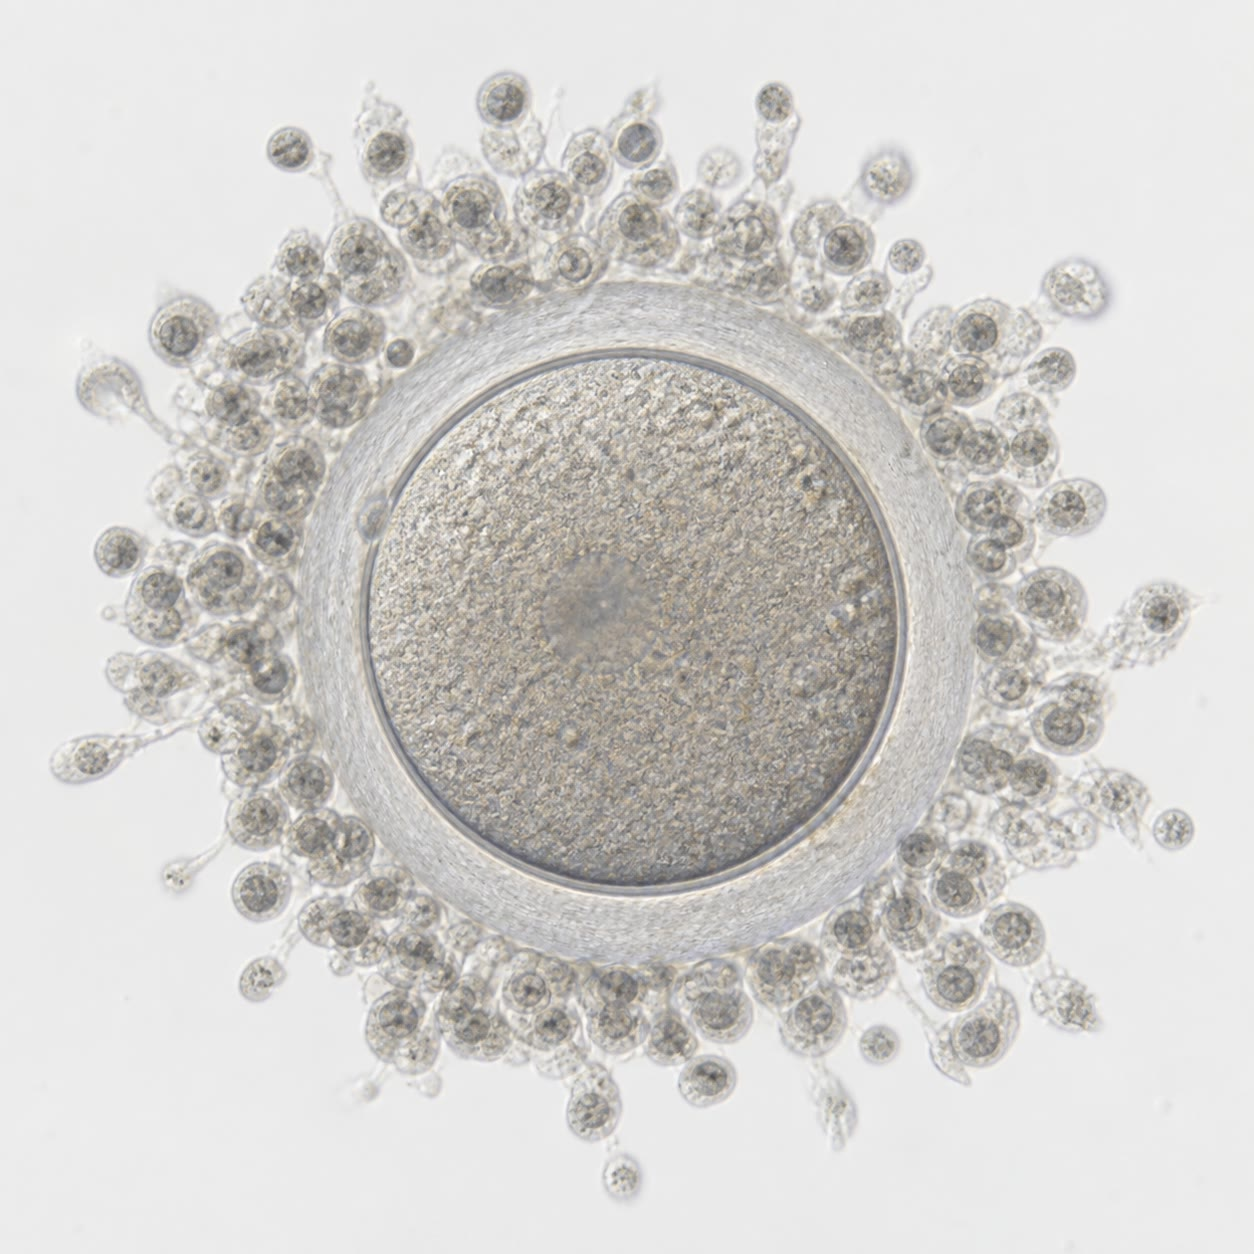
\includegraphics[width=0.46\linewidth]{images/book4/ai/b4-08-oocyte.jpg}

{\small Un ovocito ovulado: la célula, su cubierta transparente (la \omterm{prop:b2:mammal-reproduction:fertilisation}{zona
pelúcida}) y la nube de células de la granulosa que salió del \omterm{def:b2:mammal-reproduction:ovary}{folículo}
con él.}
\end{omfigure}

\section{La fecundación}

\begin{proposition}[Las etapas de la fecundación]\label{prop:b2:mammal-reproduction:fertilisation}
\index{fecundación!en los mamíferos}\index{reacción acrosómica}\index{zona pelúcida}\index{reacción cortical}
Los espermatozoides depositados en la vagina --- unos $3\times 10^{8}$ ---
atraviesan el moco cervical, las contracciones del útero los arrastran
hacia arriba y unos pocos cientos llegan en menos de una hora a la
ampolla del oviducto, donde el óvulo espera durante un día. Por el camino
los espermatozoides experimentan la \emph{capacitación}: las secreciones
del tracto femenino despojan sus membranas de proteínas de recubrimiento
y los vuelven hiperactivos. Junto al óvulo, un espermatozoide se abre paso
entre las células de la granulosa, se une a una glucoproteína de la
\emph{\omterm{prop:b2:mammal-reproduction:fertilisation}{zona pelúcida}} y experimenta la \emph{\omterm{prop:b2:mammal-reproduction:fertilisation}{reacción acrosómica}}, que
libera enzimas que abren un camino a través de la zona; su membrana se
fusiona con la del óvulo, y el núcleo del espermatozoide entra. El óvulo
responde en segundos: una onda de calcio lo recorre, y los gránulos
corticales liberan enzimas que endurecen la zona y eliminan sus
receptores de espermatozoides --- la \emph{\omterm{prop:b2:mammal-reproduction:fertilisation}{reacción cortical}}, el bloqueo
de la poliespermia. El óvulo completa la \omterm{def:b2:meiosis-heredity:meiosis}{meiosis} II, expulsa el segundo
cuerpo polar, y los dos \emph{pronúcleos} \omterm{def:b2:meiosis-heredity:meiosis}{haploides} replican su ADN, se
aproximan y entran en la primera mitosis: el cigoto tiene un día. La
especificidad de especie reside en las proteínas de la zona, y por eso un
espermatozoide de ratón no entra en un óvulo humano.
\end{proposition}
\begin{proof}[Evidencia]
Edwards y Steptoe (1978) fecundaron en una placa un ovocito humano,
extraído del ovario poco antes de la \omterm{def:b2:mammal-reproduction:ovary}{ovulación}, con espermatozoides
capacitados, cultivaron el embrión hasta las ocho células y lo
devolvieron al útero, donde se implantó y llegó a nacer: la fecundación
in vitro. Cada etapa de la secuencia anterior se había establecido antes
en el erizo de mar y en el ratón, donde pueden observarse la fusión, la
onda de calcio y la liberación de los gránulos corticales; en el ratón,
eliminar por \omterm{def:b2:genome-diversification:mutation}{mutación} una glucoproteína de la zona (ZP2 o ZP3) da óvulos
a los que los espermatozoides no pueden unirse.
\end{proof}

\begin{theorem}[Por qué un óvulo necesita millones de espermatozoides]\label{thm:b2:mammal-reproduction:poisson}
\index{poliespermia}
Si, de $N$ espermatozoides depositados, cada uno alcanza la superficie
del óvulo de forma independiente con una pequeña probabilidad $\pi$, el
número de los que llegan sigue una ley de Poisson de media $m = N\pi$, y
la probabilidad de que llegue al menos uno es
\[
P = 1 - e^{-m}.
\]
Con $N = 3\times 10^{8}$ y $\pi \approx 10^{-8}$, $m \approx 3$
y $P \approx 0.95$; con $N = 2\times 10^{7}$ (el umbral clínico de
recuento bajo), $m = 0.2$ y $P = 0.18$. La misma aritmética muestra por
qué el bloqueo de la poliespermia es indispensable: cuando
$P$ es alta, varios espermatozoides llegan con segundos de diferencia, y
un óvulo en el que entraran dos sería triploide y moriría.
\end{theorem}
\begin{proof}
Cada espermatozoide es una prueba independiente con probabilidad de éxito
$\pi$; el número de éxitos sigue una ley binomial, que para $N$ grande y
$\pi$ pequeña es una ley de Poisson de media $N\pi$. La probabilidad de
ningún éxito es $e^{-m}$, y la de al menos uno, $1 - e^{-m}$; la
probabilidad de dos o más es $1 - e^{-m}(1 + m)$, unos $0.8$ para
$m = 3$.
\end{proof}

\begin{omfigure}
\begin{tikzpicture}[every node/.style={font=\scriptsize}, >=stealth]
  \foreach \x/\lab in {0/{1. el espermatozoide\\se une a la zona}, 3.3/{2. reacción acrosómica:\\las enzimas abren paso}, 6.6/{3. fusión de membranas;\\onda de calcio}, 9.9/{4. reacción cortical:\\zona endurecida,\\meiosis II completada}} {
    \begin{scope}[xshift=\x cm]
      \draw[thick, fill=omThm!8] (0,0) circle (0.9);
      \draw[thick, omExo!70!black] (0,0) circle (1.15);
      \node[below, align=center] at (0,-1.3) {\lab};
    \end{scope}
  }
  % stage 1: sperm at zona
  \draw[thick, fill=omDef!50] (-1.45,0.1) ellipse (0.18 and 0.11); \draw[thick, omDef] (-1.63,0.1) .. controls (-2.0,0.4) and (-2.2,-0.2) .. (-2.5,0.1);
  % stage 2: sperm digging through zona
  \begin{scope}[xshift=3.3cm]
    \fill[white] (-1.2,0.0) circle (0.12);
    \draw[thick, fill=omDef!50] (-1.05,0.05) ellipse (0.18 and 0.11); \draw[thick, omDef] (-1.23,0.05) .. controls (-1.6,0.35) and (-1.8,-0.25) .. (-2.1,0.05);
    \foreach \a in {150,170,190,210} \draw[omProp, thick] (-1.2,0.0) -- ++(\a:0.25);
  \end{scope}
  % stage 3: fused, calcium wave
  \begin{scope}[xshift=6.6cm]
    \fill[white] (-1.15,0.0) circle (0.12);
    \draw[thick, fill=omDef!50] (-0.75,0.0) ellipse (0.18 and 0.11);
    \draw[thick, omDef] (-0.93,0.0) .. controls (-1.3,0.3) and (-1.5,-0.3) .. (-1.8,0.0);
    \foreach \r in {0.35,0.55,0.75} \draw[omProp, thick] (-0.75,0) ++(-60:\r) arc (-60:60:\r);
  \end{scope}
  % stage 4: hardened zona, polar body, pronuclei
  \begin{scope}[xshift=9.9cm]
    \draw[very thick, omExo!70!black] (0,0) circle (1.15);
    \draw[thick, fill=omDef!30] (-0.25,0.05) circle (0.2); \draw[thick, fill=omThm!30] (0.25,0.05) circle (0.2);
    \draw[thick, fill=omThm!20] (0.55,0.95) circle (0.12);
    \node[anchor=west] at (1.2,0.9) {cuerpo polar};
    \draw (0.45,0.05) -- (1.2,-0.35); \node[anchor=west] at (1.2,-0.35) {dos pronúcleos};
  \end{scope}
\end{tikzpicture}

{\small La fecundación en cuatro etapas: la unión a la zona, la \omterm{prop:b2:mammal-reproduction:fertilisation}{reacción
acrosómica}, la fusión y la onda de calcio, y la \omterm{prop:b2:mammal-reproduction:fertilisation}{reacción cortical}, que
cierra el óvulo a otros espermatozoides mientras termina la \omterm{def:b2:meiosis-heredity:meiosis}{meiosis}.}
\end{omfigure}

\section{La implantación y la placenta}

\begin{definition}[Segmentación, blastocisto, implantación]\label{def:b2:mammal-reproduction:implantation}
\index{blastocisto}\index{trofoblasto}\index{masa celular interna}\index{implantación}
El cigoto se divide cada doce a veinte horas sin crecer
(\emph{segmentación}) mientras desciende por el oviducto: dos células,
cuatro, ocho, una bola compacta de dieciséis (\emph{mórula}) y, hacia el
quinto día, un \emph{blastocisto} de unas cien células: una capa externa,
el \emph{trofoblasto}, alrededor de una cavidad, con un grupo de células
a un lado, la \emph{masa celular interna}. El trofoblasto construirá la
\omterm{def:b2:mammal-reproduction:placenta}{placenta} y las membranas; la masa celular interna se convertirá en el
embrión --- y, extraída en esta etapa, da células madre embrionarias. El
sexto día el blastocisto eclosiona de su zona, se adhiere al revestimiento
del útero y el trofoblasto lo invade: las células se fusionan en un
frente multinucleado que digiere el tejido materno y abre capilares
maternos, de modo que hacia el duodécimo día el embrión está enterrado en
la pared y bañado en sangre materna. Es la \emph{implantación}. Solo
tiene éxito en un útero preparado por la progesterona, en una ventana de
unos pocos días; alrededor de la mitad de las concepciones humanas
fracasan antes de esta etapa o durante ella, normalmente por errores
cromosómicos del óvulo.
\end{definition}

\begin{omfigure}
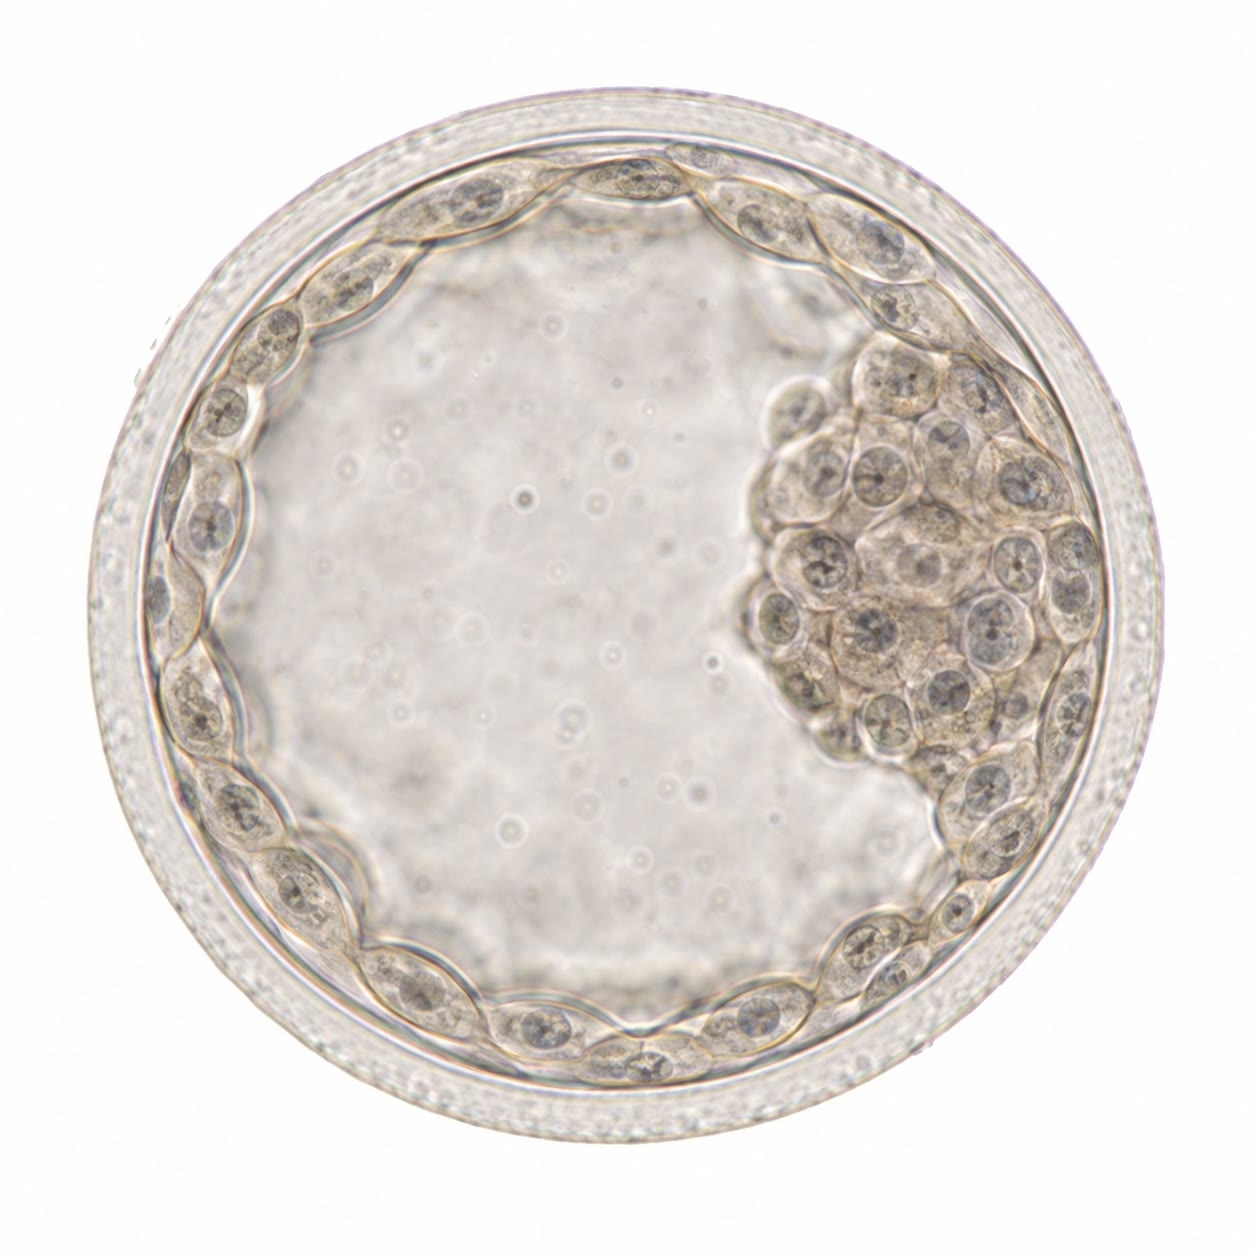
\includegraphics[width=0.42\linewidth]{images/book4/ai/b4-08-blastocyst.jpg}

{\small Un \omterm{def:b2:mammal-reproduction:implantation}{blastocisto} al quinto día: el \omterm{def:b2:mammal-reproduction:implantation}{trofoblasto} externo alrededor de
la cavidad y la \omterm{def:b2:mammal-reproduction:implantation}{masa celular interna} --- el futuro embrión --- a un lado.}
\end{omfigure}

\begin{definition}[La placenta]\label{def:b2:mammal-reproduction:placenta}
\index{placenta}\index{vellosidad coriónica}\index{cordón umbilical}
La \emph{placenta} es un órgano formado conjuntamente por el embrión (el
corion, procedente del \omterm{def:b2:mammal-reproduction:implantation}{trofoblasto}) y por la madre (el revestimiento
uterino). Unas \emph{vellosidades coriónicas} digitiformes, ramificadas
hasta alcanzar una superficie de unos \qty{12}{m^2} al término, cuelgan
en lagos de sangre materna aportada por las arterias uterinas a razón de
medio litro por minuto; dentro de cada vellosidad discurren capilares
fetales, unidos al feto a través de las dos arterias y la vena del
\emph{cordón umbilical}. Las dos sangres nunca se mezclan: las separa la
pared de la vellosidad, unos pocos micrómetros de \omterm{def:b2:mammal-reproduction:implantation}{trofoblasto} y endotelio
capilar, a través de la cual difunden el oxígeno, el
$\mathrm{CO_2}$, el agua, la urea y las moléculas liposolubles, la
glucosa y los aminoácidos pasan mediante transportadores, y los
anticuerpos maternos (IgG) son transferidos por receptores, lo que da al
recién nacido sus primeros meses de inmunidad. La placenta es también una
glándula: desde los primeros días el \omterm{def:b2:mammal-reproduction:implantation}{trofoblasto} secreta
\emph{gonadotropina coriónica humana} (hCG), que mantiene al \omterm{def:b2:mammal-reproduction:ovary}{cuerpo lúteo}
produciendo progesterona, y a partir del tercer mes la propia placenta
produce la progesterona y los estrógenos que mantienen el embarazo
(\cref{ch:b2:reproductive-hormones}). Es, en la práctica, un pulmón, un
intestino, un riñón y una glándula endocrina que crecen durante nueve
meses y se desechan en el parto.
\end{definition}
\begin{omfigure}
\begin{tikzpicture}[every node/.style={font=\scriptsize}, >=stealth]
  % maternal blood space
  \fill[omThm!12] (0,0) rectangle (8,3.6);
  \node[omThm!80!black, align=center] at (1.1,2.6) {sangre materna\\(espacio\\intervelloso)};
  % uterine wall at bottom
  \fill[omExo!30] (0,-0.6) rectangle (8,0); \node at (4,-0.3) {pared uterina (materna)};
  \draw[->, thick, omThm] (1.0,-0.6) -- (1.0,0.6); \node[omThm, anchor=west] at (1.05,0.3) {arteria espiral};
  \draw[->, thick, omDef!60!black] (7.0,0.6) -- (7.0,-0.6); \node[omDef!60!black, anchor=east] at (6.95,0.3) {vena uterina};
  % chorionic plate at top
  \fill[omDef!20] (0,3.6) rectangle (8,4.4); \node at (4,4.0) {placa coriónica (fetal)};
  % villi hanging down
  \foreach \x in {2.6,4.2,5.8} {
    \draw[thick, fill=omDef!8] (\x-0.35,3.6) -- (\x-0.4,1.4) .. controls (\x-0.4,0.9) and (\x+0.4,0.9) .. (\x+0.4,1.4) -- (\x+0.35,3.6);
    \draw[thick, omThm!70!black] (\x-0.15,3.6) -- (\x-0.15,1.5) .. controls (\x-0.15,1.25) and (\x+0.15,1.25) .. (\x+0.15,1.5) -- (\x+0.15,3.6);
    \foreach \y in {2.0,2.7} { \draw[thick, fill=omDef!8] (\x-0.4,\y) .. controls (\x-0.9,\y+0.1) and (\x-0.9,\y-0.4) .. (\x-0.4,\y-0.3); }
  }
  % umbilical vessels
  \draw[very thick, omThm!70!black] (4.2,4.4) -- (4.2,5.0) node[above, align=center] {vena umbilical (hacia el feto)\\y arterias};
  \draw[very thick, omDef!60!black] (3.9,4.4) -- (3.9,5.0); \draw[very thick, omDef!60!black] (4.5,4.4) -- (4.5,5.0);
  % exchange arrows
  \draw[<->, thick] (3.0,2.2) -- (3.75,2.2); \node[anchor=west, align=left] at (8.3,1.5) {a través de la pared: \textcolor{omThm}{O$_2$, glucosa,}\\\textcolor{omThm}{aminoácidos, IgG} hacia el feto;\\\textcolor{omDef!60!black}{CO$_2$, urea} hacia la madre};
  \node[anchor=west, align=left] at (8.3,3.0) {pared de la vellosidad: trofoblasto\\+ endotelio capilar fetal,\\unos pocos micrómetros};
  \draw (6.2,2.5) -- (8.3,3.0);
\end{tikzpicture}

{\small La \omterm{def:b2:mammal-reproduction:placenta}{placenta}: las vellosidades fetales, que llevan capilares
fetales, cuelgan en un espacio lleno de sangre materna procedente de las
arterias espirales. Las dos sangres intercambian a través de la pared de
la vellosidad y nunca se mezclan.}
\end{omfigure}

\begin{theorem}[El intercambio a través de la placenta]\label{thm:b2:mammal-reproduction:fick}
\index{ley de Fick!placenta}
Un gas que atraviesa una membrana de superficie $A$ y espesor $d$ pasa a
un ritmo $J = K\,A\,\Delta P/d$, donde $\Delta P$ es la diferencia de su
presión parcial y $K$ la permeabilidad del tejido. Para el oxígeno
en el tejido, $K \approx \qty{3e-8}{mL/(cm.min.mmHg)}$; con $A =
\qty{12}{m^2}$, $d = \qty{3.5}{\micro m}$ y $\Delta P =
\qty{20}{mmHg}$ (\qty{40}{mmHg} maternos en el espacio intervelloso
frente a \qty{20}{mmHg} en la arteria umbilical), la \omterm{def:b2:mammal-reproduction:placenta}{placenta} podría
transferir unos \qty{200}{mL} de oxígeno por minuto, unas ocho veces los
\qty{25}{mL/min} que consume un feto a término. La transferencia de
oxígeno no está limitada, por tanto, por la difusión sino por el flujo
sanguíneo; el feto trabaja a una presión de oxígeno baja y lo compensa
con una hemoglobina de mayor afinidad y un recuento de glóbulos rojos más
alto.
\end{theorem}
\begin{proof}
La ley de Fick establece que el flujo es proporcional al gradiente
$\Delta P/d$ y a la superficie; la constante $K$ engloba la solubilidad y
el coeficiente de difusión del gas en el tejido. Numéricamente:
$3\times 10^{-8}\times 1.2\times 10^{5}\times 20/(3.5\times 10^{-4})
= \qty{206}{mL/min}$ con $A$ en \unit{cm^2} y $d$ en \unit{cm}.
La demanda fetal es de unos \qty{7}{mL} por kilogramo y por minuto para
\qty{3.5}{kg}.
\end{proof}

\section{Gestación, parto y lactancia}

\begin{proposition}[Gestación y parto]\label{prop:b2:mammal-reproduction:birth}
\index{gestación}\index{parto}\index{oxitocina}
La gestación dura \num{20} días en el ratón, \num{280} en el ser humano y
\num{660} en el elefante --- aproximadamente como la potencia un cuarto de
la masa corporal, con los primates lentos para su tamaño. La mantiene la
progesterona, que mantiene en reposo el músculo uterino y cerrado el
cuello del útero. El \emph{parto} lo desencadena el propio feto: su cortisol
suprarrenal, que aumenta al término, desplaza la producción placentaria
de progesterona hacia los estrógenos, que dotan al útero de receptores de
oxitocina y de uniones comunicantes e inician la liberación de
prostaglandinas. Después toma el relevo una \emph{retroalimentación
positiva}: la cabeza presiona el cuello del útero, unos nervios
sensitivos avisan al hipotálamo, la neurohipófisis libera
\emph{oxitocina}, el útero se contrae y la cabeza presiona con más
fuerza; el bucle se intensifica hasta el nacimiento, tras el cual el
estímulo cesa y el bucle se detiene --- una de las pocas
retroalimentaciones positivas de la fisiología, y una que debe terminar
en un acontecimiento. La \omterm{def:b2:mammal-reproduction:placenta}{placenta} se expulsa minutos después.
\end{proposition}
\begin{proof}[Evidencia]
Ferguson (1941) mostró en la coneja que distender el cuello del útero
provocaba contracciones uterinas y que seccionar la médula espinal o
extirpar la neurohipófisis abolía la respuesta: un reflejo
neuroendocrino del cuello del útero a la hipófisis y de esta al útero.
La oxitocina, aislada y sintetizada por du Vigneaud en 1953, es hoy el
fármaco de referencia para inducir el parto.
\end{proof}

\begin{proposition}[La lactancia]\label{prop:b2:mammal-reproduction:lactation}
\index{lactancia}\index{prolactina}\index{leche}
La glándula mamaria, una glándula sudorípara modificada, se desarrolla
durante el embarazo por acción de los estrógenos, la progesterona y la
prolactina, pero la progesterona le impide secretar; cuando sale la
\omterm{def:b2:mammal-reproduction:placenta}{placenta}, la progesterona cae y, bajo la acción de la \emph{prolactina}
de la adenohipófisis, los alvéolos empiezan a producir leche. Dos reflejos
dirigen el proceso: la succión estimula la liberación de prolactina (que
mantiene la síntesis y suprime la \omterm{def:b2:mammal-reproduction:ovary}{ovulación}) y la de oxitocina (que
contrae las células que rodean los alvéolos y expulsa la leche). La leche
humana contiene alrededor de un \qty{7}{\%} de lactosa, un \qty{4}{\%} de
grasa y un \qty{1}{\%} de proteína, y aporta
\qty{2.9}{kJ/mL}; el \emph{calostro} de los primeros días es rico en
anticuerpos (IgA) que recubren el intestino del lactante. Una madre
produce unos \qty{750}{mL} al día, con un coste de unos \qty{2.5}{MJ} ---
una cuarta parte de su alimento --- durante meses; la lactancia es la
parte más cara de la reproducción de los mamíferos y la que da nombre a
la clase.
\end{proposition}

\section{La formación de los dos sexos}

\begin{proposition}[Determinación y diferenciación del sexo]\label{prop:b2:mammal-reproduction:sex}
\index{SRY}\index{hormona antimülleriana}\index{diferenciación sexual}
Hasta la sexta semana, un embrión humano de cualquier sexo tiene el mismo
equipamiento: una gónada indiferenciada, dos pares de conductos (de
\emph{Wolff} y de \emph{Müller}) y unos genitales externos neutros. El gen
\emph{SRY} del cromosoma Y se activa en la gónada y la convierte en
\omterm{def:b2:mammal-reproduction:testis}{testículo}; sin él, la gónada se convierte en ovario. El \omterm{def:b2:mammal-reproduction:testis}{testículo} fetal
hace entonces dos cosas: sus \omterm{def:b2:mammal-reproduction:testis}{células de Sertoli} secretan la
\emph{\omterm{prop:b2:mammal-reproduction:sex}{hormona antimülleriana}}, que hace regresar los conductos de Müller,
y sus \omterm{def:b2:mammal-reproduction:testis}{células de Leydig} secretan \emph{testosterona}, que mantiene los
conductos de Wolff (el futuro epidídimo, conducto deferente y vesículas
seminales) y, convertida en dihidrotestosterona, modela los genitales
externos en pene y escroto. En ausencia de ambas señales, los conductos
de Wolff regresan, los conductos de Müller se convierten en los
oviductos, el útero y la parte superior de la vagina, y los genitales se
desarrollan como femeninos. La vía femenina es la que se sigue cuando no
se dice nada: la vía masculina debe imponerla activamente el \omterm{def:b2:mammal-reproduction:testis}{testículo},
y cada etapa en la que la imposición falla --- un SRY mutante, un
receptor hormonal ausente --- da un individuo XY con un cuerpo femenino
o intermedio.
\end{proposition}
\begin{proof}[Evidencia]
Jost (1947) extirpó las gónadas de fetos de conejo dentro del útero antes
de que sus conductos se diferenciaran: los fetos castrados de cualquier
sexo cromosómico desarrollaron útero, oviductos y genitales femeninos. Un
cristal de testosterona implantado en un feto castrado mantenía los
conductos de Wolff de ese lado, pero no eliminaba los conductos de
Müller; un \omterm{def:b2:mammal-reproduction:testis}{testículo} fetal injertado hacía ambas cosas, en su propio
lado: el \omterm{def:b2:mammal-reproduction:testis}{testículo} debía producir un segundo factor, entonces
desconocido, para suprimir los conductos femeninos, identificado treinta
años después como la \omterm{prop:b2:mammal-reproduction:sex}{hormona antimülleriana}. Más tarde, el efecto de
inversión sexual de un pequeño fragmento del cromosoma Y localizó el
interruptor en \emph{SRY} (1990), y un ratón XX al que solo se añadió el
gen \emph{Sry} se desarrolló como macho.
\end{proof}

\begin{omfigure}
\begin{tikzpicture}[every node/.style={font=\scriptsize}, >=stealth]
  \node[draw, rounded corners, fill=omExo!25, align=center] (g) at (0,0) {gónada indiferenciada\\dos sistemas de conductos};
  \node[draw, rounded corners, fill=omDef!15, align=center] (t) at (4.2,1.4) {testículo\\(\emph{SRY} presente)};
  \node[draw, rounded corners, fill=omThm!15, align=center] (o) at (4.2,-1.4) {ovario\\(sin \emph{SRY})};
  \node[draw, rounded corners, fill=omDef!15, align=center] (amh) at (8.6,2.3) {AMH: regresión de los conductos de Müller};
  \node[draw, rounded corners, fill=omDef!15, align=center] (tst) at (8.6,0.6) {testosterona: se mantienen los conductos de Wolff;\\DHT: genitales externos masculinos};
  \node[draw, rounded corners, fill=omThm!15, align=center] (f) at (8.6,-1.4) {sin señal: regresión de los conductos de Wolff,\\conductos de Müller $\to$ oviductos, útero;\\genitales femeninos};
  \draw[->, thick] (g) -- (t); \draw[->, thick] (g) -- (o);
  \draw[->, thick] (t) -- (amh); \draw[->, thick] (t) -- (tst); \draw[->, thick] (o) -- (f);
\end{tikzpicture}

{\small \omterm{prop:b2:mammal-reproduction:sex}{Diferenciación sexual}: el \omterm{def:b2:mammal-reproduction:testis}{testículo}, formado por acción de
\emph{SRY}, impone la vía masculina con dos hormonas; en su ausencia, el
cuerpo se desarrolla como femenino.}
\end{omfigure}

\section{Ejercicios}

\begin{exercise}[$\star$]\label{exo:b2:mammal-reproduction:1}
Compárense la \omterm{def:b2:mammal-reproduction:testis}{espermatogénesis} y la \omterm{def:b2:mammal-reproduction:ovary}{ovogénesis}: cuándo se dividen las
células madre, cuántos gametos da una \omterm{def:b2:meiosis-heredity:meiosis}{meiosis}, cuánto se tarda en
formar un gameto, dónde están las detenciones y cuántos gametos se
producen a lo largo de la vida.
\end{exercise}

\begin{exercise}[$\star$]\label{exo:b2:mammal-reproduction:2}
Enumérense las etapas de la fecundación desde la llegada de un
espermatozoide a la \omterm{prop:b2:mammal-reproduction:fertilisation}{zona pelúcida} hasta la primera mitosis, y dígase qué
etapa bloquea la poliespermia.
\end{exercise}

\begin{exercise}[$\star$]\label{exo:b2:mammal-reproduction:3}
Nómbrense las dos poblaciones celulares del \omterm{def:b2:mammal-reproduction:implantation}{blastocisto} y el destino de
cada una. ¿Qué día empieza la \omterm{def:b2:mammal-reproduction:implantation}{implantación}, y qué hormona debe haber
preparado el útero?
\end{exercise}

\begin{exercise}[$\star$]\label{exo:b2:mammal-reproduction:4}
Para cada uno de los siguientes, dígase si atraviesa la \omterm{def:b2:mammal-reproduction:placenta}{placenta} y cómo:
oxígeno, glucosa, glóbulos rojos maternos, anticuerpos IgG, urea,
alcohol, la mayoría de las bacterias.
\end{exercise}

\begin{exercise}[$\star\star$]\label{exo:b2:mammal-reproduction:5}
Con $\pi = 10^{-8}$ por espermatozoide, calcúlese la probabilidad de
fecundación para recuentos de $3\times 10^{8}$, $10^{8}$,
$4\times 10^{7}$ y $10^{7}$ espermatozoides. ¿Con qué recuento cae por
debajo de un medio? ¿Qué dice esto sobre la forma de la relación
dosis--respuesta entre fertilidad y recuento espermático?
\end{exercise}

\begin{exercise}[$\star\star$]\label{exo:b2:mammal-reproduction:6}
Una niña nace con $10^{6}$ ovocitos, tiene \num{300000} en la pubertad
(a los 13 años) y unos \num{1000} a los 50, habiendo ovulado \num{400}.
Calcúlese el ritmo medio de atresia (ovocitos perdidos por día) antes y
después de la pubertad, y compárese con el ritmo de \omterm{def:b2:mammal-reproduction:ovary}{ovulación}.
\end{exercise}

\begin{exercise}[$\star\star$]\label{exo:b2:mammal-reproduction:7}
La hemoglobina fetal tiene una presión de semisaturación $P_{50} =
\qty{19}{mmHg}$; la adulta, \qty{27}{mmHg}; tómese la saturación como
$S = P^{n}/(P_{50}^{n} + P^{n})$ con $n = 2.7$. Calcúlense ambas
saturaciones a \qty{30}{mmHg}, la presión de la vena umbilical, y
explíquese la ventaja.
\end{exercise}

\begin{exercise}[$\star\star$]\label{exo:b2:mammal-reproduction:8}
La hCG aparece en la sangre materna en la \omterm{def:b2:mammal-reproduction:implantation}{implantación} (día 7 tras la
fecundación) a alrededor de \qty{1}{IU/L} y se duplica cada dos días;
una prueba de embarazo detecta \qty{25}{IU/L}. ¿Qué día tras la
fecundación da positivo la prueba? ¿Qué día tras la última menstruación
(\omterm{def:b2:mammal-reproduction:ovary}{ovulación} el día 14)?
\end{exercise}

\begin{exercise}[$\star\star$]\label{exo:b2:mammal-reproduction:9}
Vuélvase a calcular la transferencia placentaria de oxígeno del teorema
para una \omterm{def:b2:mammal-reproduction:placenta}{placenta} de \qty{6}{m^2} con una pared de las vellosidades de
\qty{10}{\micro m}, como en algunas patologías, y compárese con la demanda
fetal. ¿Qué le ocurre al feto?
\end{exercise}

\begin{exercise}[$\star\star\star$]\label{exo:b2:mammal-reproduction:10}
Predíganse el sistema de conductos y los genitales externos de: (a) un
feto XY cuyas células carecen del receptor de testosterona; (b) un feto
XY sin \omterm{prop:b2:mammal-reproduction:sex}{hormona antimülleriana}; (c) un feto XX expuesto a una testosterona
elevada procedente de sus suprarrenales; (d) un feto XX que lleva
\emph{SRY} en un cromosoma X. Explíquese cada caso a partir de los
resultados de Jost.
\end{exercise}

\begin{exercise}[$\star\star\star$]\label{exo:b2:mammal-reproduction:11}
Los gemelos idénticos se forman cuando un embrión se divide. Si se divide
antes del día 3, los gemelos tienen \omterm{def:b2:mammal-reproduction:placenta}{placentas} y sacos separados; entre
los días 4 y 8, una \omterm{def:b2:mammal-reproduction:placenta}{placenta} y dos sacos; entre los días 8 y 13, una
\omterm{def:b2:mammal-reproduction:placenta}{placenta} y un saco; más tarde, son siameses. En una serie de gemelos
idénticos, el \qty{30}{\%} tiene \omterm{def:b2:mammal-reproduction:placenta}{placentas} separadas, el \qty{68}{\%} una
\omterm{def:b2:mammal-reproduction:placenta}{placenta} y dos sacos, y el \qty{2}{\%} un saco. Dedúzcase qué estadio del
desarrollo se divide con más frecuencia, y explíquese en términos del
\omterm{def:b2:mammal-reproduction:implantation}{blastocisto} qué estructuras se comparten en cada caso.
\end{exercise}

\begin{exercise}[$\star\star\star$]\label{exo:b2:mammal-reproduction:12}
Los marsupiales paren al cabo de unas pocas semanas una cría del tamaño
de una judía que completa su crecimiento sobre un pezón, en la bolsa; los
mamíferos placentarios tienen una gestación larga y paren una cría
grande. Compárense las dos estrategias en términos de coste materno, de
riesgo y de la capacidad de la madre para abandonar una camada en una
mala estación, y propóngase por qué los placentarios han desplazado a los
marsupiales en todos los continentes salvo Australia.
\end{exercise}

\section{Problema: un embarazo en cifras}

\begin{problem}[{Problema de fin de semana --- un embarazo humano seguido
desde el espermatozoide hasta la leche, a través de las probabilidades de
fecundación, el calendario de la implantación y su hormona, la capacidad
de intercambio de la placenta y el coste energético de la gestación y la
lactancia, hasta llegar a la probabilidad de fecundación, el día en que
la prueba da positivo, el margen de oxígeno de la placenta y el coste de
un día de leche}]
\label{pb:b2:mammal-reproduction:1}
Datos: $3\times 10^{8}$ espermatozoides por eyaculación, cada uno de los
cuales llega al óvulo con probabilidad $10^{-8}$; los espermatozoides
nadan a \qty{50}{\micro m/s}; la ampolla está a \qty{15}{cm} del cuello
del útero. hCG en la \omterm{def:b2:mammal-reproduction:implantation}{implantación} (día 7):
\qty{1}{IU/L}, que se duplica cada \qty{2}{d}; umbral de la prueba,
\qty{25}{IU/L}. \omterm{def:b2:mammal-reproduction:placenta}{Placenta} al término: \qty{12}{m^2}, pared de
\qty{3.5}{\micro m}, $K_{\mathrm{O_2}} = \qty{3e-8}{mL/(cm.min.mmHg)}$,
$\Delta P = \qty{20}{mmHg}$; feto de \qty{3.5}{kg} que consume
\qty{7}{mL} de oxígeno por kilogramo y por minuto; flujo sanguíneo
placentario materno de \qty{500}{mL/min}, con \qty{0.16}{mL} de oxígeno
por mililitro de sangre. Glucosa: el feto usa \qty{5}{mg} por kilogramo y
por minuto; sangre materna a \qty{0.9}{g/L}. Leche: \qty{750}{mL/d} a
\qty{2.9}{kJ/mL}, producida con un rendimiento del \qty{80}{\%}; el
lactante gana \qty{30}{g/d} de tejido a \qty{6}{kJ/g} depositados y gasta
\qty{300}{kJ/kg/d} en mantenimiento a \qty{4}{kg}.

\medskip
\noindent\textbf{Parte I --- La fecundación.}
\begin{enumerate}
  \item Calcúlense el número medio de espermatozoides que llegan al óvulo
        y la probabilidad de fecundación.
  \item Calcúlese la probabilidad de que lleguen dos o más, y dígase qué
        ocurriría sin la \omterm{prop:b2:mammal-reproduction:fertilisation}{reacción cortical}.
  \item ¿Cuánto tardaría un espermatozoide en llegar nadando a la
        ampolla? Se encuentran espermatozoides allí en menos de
        \qty{30}{min}: ¿qué los transporta?
  \item Solo unos pocos cientos de espermatozoides llegan a la ampolla.
        ¿Qué fracción de la eyaculación es esa, y dónde se pierden los
        demás?
  \item Un óvulo es fecundable durante un día aproximadamente, y los
        espermatozoides sobreviven unos tres días en el tracto. ¿Durante
        cuántos días del ciclo pueden las relaciones sexuales dar lugar a
        una concepción?
  \item El recuento de un hombre cae a $5\times 10^{7}$. Vuélvanse a
        calcular la probabilidad de fecundación por ciclo y el número
        esperado de ciclos hasta la concepción (ley geométrica).
  \item Explíquese por qué es el óvulo, y no el espermatozoide, el que
        aporta las mitocondrias del embrión.
\end{enumerate}

\medskip
\noindent\textbf{Parte II --- La \omterm{def:b2:mammal-reproduction:implantation}{implantación} y su hormona.}
\begin{enumerate}[resume]
  \item ¿Cuántas divisiones de segmentación se han producido hacia el
        día 5 si cada una dura \qty{16}{h}? ¿Cuántas células hay?
  \item ¿Qué día tras la fecundación alcanza la hCG el umbral de la
        prueba? ¿Y tras la última regla (\omterm{def:b2:mammal-reproduction:ovary}{ovulación} el día 14)?
  \item ¿Por qué debe aparecer la hCG pocos días después de la
        \omterm{def:b2:mammal-reproduction:implantation}{implantación}? ¿Qué le ocurre al \omterm{def:b2:mammal-reproduction:ovary}{cuerpo lúteo}, y al embarazo, si no
        aparece?
  \item La hCG alcanza un máximo cercano a \qty{1e5}{IU/L} hacia la
        semana 10 y después disminuye. ¿Cuántas duplicaciones desde la
        \omterm{def:b2:mammal-reproduction:implantation}{implantación} supone eso, y por qué puede disminuir después sin que
        se pierda el embarazo?
  \item La mitad de las concepciones se pierden antes de la \omterm{def:b2:mammal-reproduction:implantation}{implantación}
        o durante ella, sobre todo por óvulos aneuploides. Explíquese, con
        el calendario de la \omterm{def:b2:mammal-reproduction:ovary}{ovogénesis}, por qué la aneuploidía es más
        frecuente en los óvulos que en los espermatozoides.
  \item Gemelos: un embrión que se divide el día 6. Dígase si los gemelos
        comparten la \omterm{def:b2:mammal-reproduction:placenta}{placenta} y el saco amniótico.
\end{enumerate}

\medskip
\noindent\textbf{Parte III --- La \omterm{def:b2:mammal-reproduction:placenta}{placenta}.}
\begin{enumerate}[resume]
  \item Calcúlese la transferencia difusiva máxima de oxígeno.
  \item Calcúlense la demanda fetal de oxígeno y el margen de difusión.
  \item Calcúlese el oxígeno aportado por minuto por el flujo sanguíneo
        materno a la \omterm{def:b2:mammal-reproduction:placenta}{placenta}. ¿Qué fracción debe extraerse para cubrir la
        demanda?
  \item Calcúlense la demanda fetal de glucosa en gramos por día y el
        volumen de sangre materna que la contiene. Compárese con el flujo
        placentario materno diario.
  \item La sangre del feto sale de la \omterm{def:b2:mammal-reproduction:placenta}{placenta} a \qty{30}{mmHg} de
        oxígeno. ¿Por qué no se asfixia a una presión que dejaría
        inconsciente a un adulto?
  \item Nómbrense dos cosas que hace la \omterm{def:b2:mammal-reproduction:placenta}{placenta} y que ningún otro órgano
        del embrión podría hacer en ese momento, y una que no puede hacer.
\end{enumerate}

\medskip
\noindent\textbf{Parte IV --- El parto y la leche.}
\begin{enumerate}[resume]
  \item Descríbase la retroalimentación positiva del parto y explíquese
        por qué no se desencadena antes del término.
  \item Calcúlense la energía contenida en la leche de un día y la energía
        que gasta la madre para producirla.
  \item Calcúlese el balance energético diario del lactante (crecimiento
        más mantenimiento) y compárese con la leche aportada.
  \item Calcúlese el coste energético total para la madre de nueve meses
        de lactancia, y compárese con los \qty{300}{MJ} que cuesta el
        propio embarazo.
  \item Explíquese por qué la succión retrasa el retorno de la
        \omterm{def:b2:mammal-reproduction:ovary}{ovulación}, y por qué esto importa en las poblaciones sin
        anticoncepción.
  \item Enúnciese el resultado: la probabilidad de fecundación, el día en
        que la prueba da positivo, el margen de oxígeno de la \omterm{def:b2:mammal-reproduction:placenta}{placenta} y el
        coste de un día de leche.
\end{enumerate}
\end{problem}
